\documentclass[11pt,a4paper]{article}
\usepackage[utf8]{inputenc}
\usepackage[T1]{fontenc}
\usepackage{lmodern}
\usepackage[margin=24mm]{geometry}
\usepackage{amsmath,amssymb,graphicx,booktabs,longtable,array}
\usepackage[hidelinks]{hyperref}
\usepackage{microtype}
\graphicspath{{../figures/}}
\setlength{\parskip}{5pt}
\setlength{\parindent}{0pt}
\newcommand{\doctype}{Technical report (local draft)}
\newcommand{\docversion}{0.23.000}
\newcommand{\docdate}{1 November 2026}
\newcommand{\versiondoi}{Not assigned; publication pending}
\newcommand{\conceptdoi}{Not assigned; separate record required}
\newcommand{\docrepo}{github.com/fsantibanezleal/CAOS\_RES\_ChronoScope}
\newcommand{\headerblock}{\begin{center}\fbox{\parbox{0.94\textwidth}{\small\raggedright
\textbf{\doctype}\quad v\docversion, \docdate\quad Licence CC BY 4.0\\[2pt]
CAOS open-research programme; ChronoScope forecasting and diagnostic atlas.\\[2pt]
Version DOI: \versiondoi. Concept DOI (always latest): \conceptdoi.\\[2pt]
Not peer reviewed. Source, data and computational records: \url{https://github.com/fsantibanezleal/CAOS_RES_ChronoScope}.
}}\end{center}}
\title{ChronoScope: Forecasting Implementations, Contiguous-History Evaluation and Context-Dependent Combination}
\author{Felipe Santib\'a\~nez-Leal\\CAOS open-research programme, Santiago, Chile\\\small ORCID: 0000-0002-0150-3246}
\date{}
\begin{document}
\maketitle
\headerblock
\begin{abstract}
Forecast comparisons are useful only when their information sets, implementation identities and scoring targets are explicit. ChronoScope combines a diagnostic atlas with a reproducible forecasting workbench. Its current final-block experiment compares twenty-two variants on fifteen selected series: fourteen released model paths are rescored, five corrected lightweight methods execute on reconstructed contiguous histories, and a context-dependent combination is evaluated against matching recency-only and equal-weight ablations. Two algorithm defects were corrected: additive HoltWinters seasonal continuation after an incomplete cycle, and a finite-history term in Theta. A separate evaluation defect was identified and invalidated: display-decimated replay histories had been used as consecutive fitting observations. Reconstructing the original observations changes the historical scales and the recomputed predictions. Under the corrected protocol, ContextMemory has mean MASE 1.4504, compared with 1.4489 for RecencyMean and 1.8970 for EqualMean. The additional context component therefore fails its declared aggregate criterion. A source-bound artifact, normative schemas, generated browser types and eight executed bilingual lessons make the implementation and its limits inspectable. One origin per selected series, historical heavy-model inference and unverified pretraining overlap preclude population superiority or deployment claims.
\end{abstract}

\section{Decision problem and scope}
Inventory, staffing and capacity commitments depend on forecasts made before demand is observed. A forecast revision can alter those commitments even when its statistical benefit has not been measured. The relevant engineering question is therefore broader than selecting the smallest displayed error: which observations were available, what algorithm produced the path, which future outcomes were scored, and what uncertainty remains before an action is taken?

ChronoScope supports inspection of these questions through selected real excerpts, generated mechanisms and explicit controls. Generated cases explain mechanisms and expose defects; they are not customer observations. The real excerpts represent electricity demand, air quality and M4 series. Air quality is a forecasting example rather than a demand-planning measurement. No monetary benefit, service-level improvement, laboratory result or customer deployment is inferred from these examples.

The browser offers series structure, forecasts, interval boundaries, individual errors and historical streaming diagnostics. Documentation separates a sourced executive problem framing from technical method descriptions. The product is a research and teaching instrument. Acceptance of a production policy would additionally require an operational objective, representative data, governance of revisions, latency constraints and prospective evaluation.

\section{Implementation identities}
The method roster distinguishes algorithms from their implementations. A reference library, a direct adaptation and a small browser-exported model can share an architectural idea while differing in objectives, preprocessing and training budget. Their results remain separate.

\begin{longtable}{p{0.22\textwidth}p{0.32\textwidth}p{0.37\textwidth}}
\toprule Methods & Implementation and settings & Evidence in the common experiment\\\midrule\endhead
SeasonalNaive, SES, Holt, HoltWinters, Theta & NumPy core; browser TypeScript parity; finite smoothing grids & Recomputed on original contiguous prefixes. Gaussian residual intervals are approximations.\\
AutoETS, AutoTheta, AutoARIMA & statsforecast; ARIMA stepwise and approximate, context cap 360 & Released paths rescored. Separate worked lessons freshly execute the installed adapters.\\
LightGBM & MLForecast lag table; 100 trees, 31 leaves, learning rate 0.05, context cap 500 & Released point-regression path rescored; Gaussian residual intervals. A lesson freshly executes the adapter.\\
NLinear, DLinear, NHITS & Direct-torch quantile-head adaptations & Released paths rescored; not asserted to be exact replications of the papers.\\
NLinear (nf), DLinear (nf), NHITS (nf) & neuralforecast reference implementations; fixed 300-step training budget & Released paths rescored; the budget is part of the experiment.\\
Chronos-Bolt, Chronos-2, TimesFM 2.5, TiRex-2 & Pretrained checkpoint adapters; TiRex bridge uses WSL/CUDA & Released paths rescored, without current-checkpoint or pretraining-independence claims.\\
ContextMemory, RecencyMean, EqualMean & Same five light experts; fixed causal memory and two ablations & Newly computed with matching original prefixes and final targets.\\\bottomrule
\end{longtable}

An additional browser NLinear model is exported to ONNX after least-squares fitting on generated windows. It predicts twelve observations from a forty-eight-observation context. It is an independently identified live demonstration, not an additional member of the twenty-two-variant aggregate experiment. On real cases its first twelve held-out targets can be inspected without adapting the fit to those targets. Its interval scale is inherited from its training metadata and does not establish calibration on the real excerpts.

\subsection{Corrected lightweight methods}
SeasonalNaive repeats the latest observed cycle. SES updates a level, Holt adds a trend, and additive HoltWinters additionally updates a seasonal component. At a prefix length $n$, the seasonal slot for zero-based future lead $k$ must continue as $(n+k)\bmod m$. Restarting at $k\bmod m$ is incorrect when $n$ is not a multiple of $m$. An adversarial partial-season example tests this condition independently in Python; the browser parity fixture includes a non-multiple history and a horizon longer than one cycle.

For the nonseasonal Theta implementation, the corrected point equation is
\begin{equation}
\widehat y_{n+h}=\ell_n+\frac{b}{2}\left[h-1+\frac{1-(1-\alpha)^n}{\alpha}\right],\qquad h\geq1,
\end{equation}
where $\ell_n$ is the selected SES level and $b$ is the fitted linear slope. An independent two-Theta-line construction verifies the finite-history term following Hyndman and Billah~\cite{theta}. This local method does not inherit AutoTheta's automatic seasonal adjustment merely because the names are related.

The Gaussian widening rule maps a residual standard deviation to three ordered columns at probabilities 0.1, 0.5 and 0.9. Residual estimation, Gaussian shape and horizon widening are assumptions. Neither an ordered matrix nor a quantile-loss fit establishes marginal or conditional calibration. These distinctions also apply to the direct neural adaptations and the lag-tree adapter.

\section{Diagnostic atlas and computational boundaries}
The diagnostic toolkit contains ten families: stationarity, autocorrelation, seasonality, filtering and decomposition, change points, volatility, distribution and complexity, fractals, nonlinear dynamics, and causality. Methods include ADF/KPSS and related tests, ACF/PACF and Ljung--Box diagnostics, STL/MSTL and periodograms, offline change-point procedures, ARCH/GARCH diagnostics and surrogate-based nonlinear analyses. A short series or unavailable dependency produces an explicit unavailable result for that analysis; it does not silently produce a substitute measurement.

Statistical diagnostics are descriptive or model-dependent. An autocorrelation band containing the observed coefficients does not prove white noise. A unit-root test does not certify future stationarity. A fractal estimate is sensitive to sample length, detrending and the assumed stochastic class. A nonlinear surrogate rejection does not uniquely identify deterministic chaos. The workbench exposes these cautions alongside the results rather than presenting a diagnostic label as a forecasting guarantee.

The browser recomputes lightweight diagnostics and light forecasts for generated scenarios. Committed analysis artifacts retain their original scope; several describe the complete observed series, including what later becomes a forecasting holdout. They are suitable for retrospective explanation, not for feature selection at the earlier forecast origin. The proposed combination computes its own prefix-only contexts and does not consume those retrospective diagnostics.

Heavy statistical, neural and pretrained calculations run offline. GPU availability, checkpoint caches and Python environments are distinct from the served browser bundle. A local environment with only NumPy cannot be represented as a complete neural or foundation-model rerun. Conversely, rescoring a stored model path does not require pretending that its original runtime has been restored.

\section{Data provenance and temporal reconstruction}
The corpus contains eleven generated cases and four real excerpts. Generated mechanisms cover seasonality, trend, intermittent arrivals, a level shift, multiple seasonalities, heteroscedasticity, long memory, a delayed nonlinear system and a known-future exogenous driver. White noise and a near-random walk remain visible as controls. The exogenous-driver comparison requires a declared arrival policy; univariate forecasts do not gain access to future covariates automatically.

\begin{longtable}{lrrrl}
\caption{Admitted case inventory with original contiguous history length, forecast horizon, seasonal lag and source class; generated mechanisms remain distinct from authentic observations.}\label{tab:cases}\\
\toprule Case & History & Horizon & Lag & Source\\\midrule\endfirsthead
\toprule Case & History & Horizon & Lag & Source\\\midrule\endhead
BRKV\_level\_shift & 288 & 12 & 12 & Generated\\
CHAO\_mackey & 488 & 12 & 1 & Generated\\
CTRL\_white\_noise & 148 & 12 & 1 & Generated\\
EXOG\_promo & 226 & 14 & 7 & Generated\\
HETV\_garch & 488 & 12 & 1 & Generated\\
INTM\_demand & 188 & 12 & 1 & Generated\\
LMEM\_fractional & 488 & 12 & 1 & Generated\\
MSEA\_daily\_weekly & 648 & 24 & 24 & Generated\\
REAL\_electricity & 456 & 24 & 24 & Real excerpt\\
REAL\_m4\_daily & 386 & 14 & 7 & Real excerpt\\
REAL\_m4\_hourly & 456 & 24 & 24 & Real excerpt\\
REAL\_pm25 & 456 & 24 & 24 & Real excerpt\\
RWLK\_noise & 188 & 12 & 1 & Generated\\
SEAS\_hourly & 456 & 24 & 24 & Generated\\
TRND\_seasonal & 168 & 12 & 12 & Generated\\
\bottomrule
\end{longtable}


The source manifest records provenance, redistribution permission, seed, original series descriptors, artifact paths and byte counts. Real-data CSVs are committed as compact admitted excerpts. A source's redistribution status is an explicit field; a restricted source must not expose its raw path merely because aggregate metrics are publishable. The current comparison uses only available, non-redacted inputs.

\subsection{Why a replay history is not a fitting series}
The released trace stores at most three hundred historical display samples and their original indices. Nine case histories exceed that display limit. Treating those samples as consecutive observations changes the time interval and can destroy the meaning of a seasonal lag. It also changes a historical scale used by MASE. The initial comparison made this error and is invalidated; its earlier bytes remain identifiable through Git, not as admitted scientific evidence.

The corrected protocol reconstructs the original series from each committed CSV or deterministic case definition and its manifest seed. At every displayed index the reconstructed observation must agree with the released rounded value within 0.000051. The final targets must also agree at that tolerance, and the original prefix length must match the trace's declared history length. All fifteen reconstructions satisfy these checks. The complete contiguous prefix is used for light fitting and historical scaling. Original per-engine context caps remain explicit; a common available prefix does not mean every algorithm consumes the same number of observations.

The reconstructed history retains source precision. Frozen targets and model paths retain their released four-decimal precision. This small rounding distinction is disclosed and is not the much larger temporal-decimation error. Source and implementation hashes bind the corrected artifact to the exact inputs. A replay-only array whose declared length exceeds its display length is refused as a consecutive fit input.

\section{Common final-block protocol}
Each selected series supplies one forecast origin and one final block. Fourteen heavy forecast paths remain frozen; five corrected lightweight methods and three combinations are newly computed. Every admitted path is scored on the same actual values and horizon within its case. Original rolling-backtest results remain archived. Their differing origin budgets, ranging from three to more than twenty-five windows, make a direct ranking of those aggregates confounded by the evaluation schedule.

Let $y_1,\ldots,y_n$ denote the contiguous prefix, $a_1,\ldots,a_H$ the final targets and $p_j$ a point prediction. The historical seasonal scale is
\begin{equation}
s_m=\frac{1}{n-m}\sum_{t=m+1}^{n}|y_t-y_{t-m}|,
\end{equation}
with the lag bounded to the available history. MAE is $H^{-1}\sum_j|a_j-p_j|$, RMSE is the square root of mean squared error, and MASE is MAE$/s_m$~\cite{mase}. A value below one compares a future error with a historical scale. It does not directly show that the method beat an independently scored SeasonalNaive path on the same future block. A zero scale produces an unavailable scaled metric rather than an invented denominator.

For lower and upper columns $l_j,u_j$, empirical coverage is $H^{-1}\sum_j\mathbf1\{l_j\leq a_j\leq u_j\}$ and width is $H^{-1}\sum_j(u_j-l_j)$. With nominal interval miscoverage $\alpha=0.2$, the interval score is
\begin{equation}
IS_j=(u_j-l_j)+\frac{2}{\alpha}(l_j-a_j)_++\frac{2}{\alpha}(a_j-u_j)_+.
\end{equation}
MSIS is its block mean divided by $s_m$. The artifact's WQL uses only $Q=\{0.1,0.5,0.9\}$:
\begin{equation}
\mathrm{WQL}_3=\frac{2\sum_{q\in Q}\sum_{j=1}^H\rho_q(a_j-\widehat y_j^{(q)})}{3\sum_{j=1}^H|a_j|},\quad
\rho_q(e)=\max(qe,(q-1)e).
\end{equation}
This is an average of three quantile losses, not a complete predictive-density evaluation. A zero absolute-target sum makes this normalized score unavailable. Proper-score theory motivates reporting probabilistic quality, while the finite quantile grid limits what is observed~\cite{scores}.

\section{A fixed context-memory proposal}
ContextMemory tests whether similar completed historical contexts help estimate expert competence beyond recency alone. Feature-dependent combinations and dynamic ensembles are established ideas~\cite{fforma,ade}. The experiment tests a specific within-series recurrence rule and makes no priority claim for contextual weighting.

The expert set is fixed to SeasonalNaive, SES, Holt, HoltWinters and Theta. Up to twelve completed historical origins are selected within the prefix. For every origin $o$, eligibility requires $o+H\leq n$. A normalized slope, level shift, volatility-change statistic and seasonal correlation describe the context. Expert multi-step absolute losses are normalized using information available at that origin. A Gaussian context-distance kernel combines with recency weights of half-life six origins. Local estimated losses are shrunk 25\% toward the recency-only loss estimate.

An exponential loss transformation produces a simplex allocation, followed by a 5\% uniform floor. With $K=5$ experts, each final weight is at least $0.05/K=0.01$ and the weights sum to one. Corresponding point and quantile columns are averaged with these same weights. Nonnegative convex weights preserve the order of the input quantile columns. They do not make the result a calibrated predictive mixture.

RecencyMean removes context similarity while retaining the experts, historical origins, recency weighting and competence transformation. EqualMean assigns a uniform allocation. These matching ablations distinguish the contextual component from the more general benefit of combining methods. A positive scale and location transformation supplies a structural check away from numerical degeneracy thresholds. Completed-target eligibility and quantile ordering have independent adversarial tests.

\begin{figure}[htbp]\centering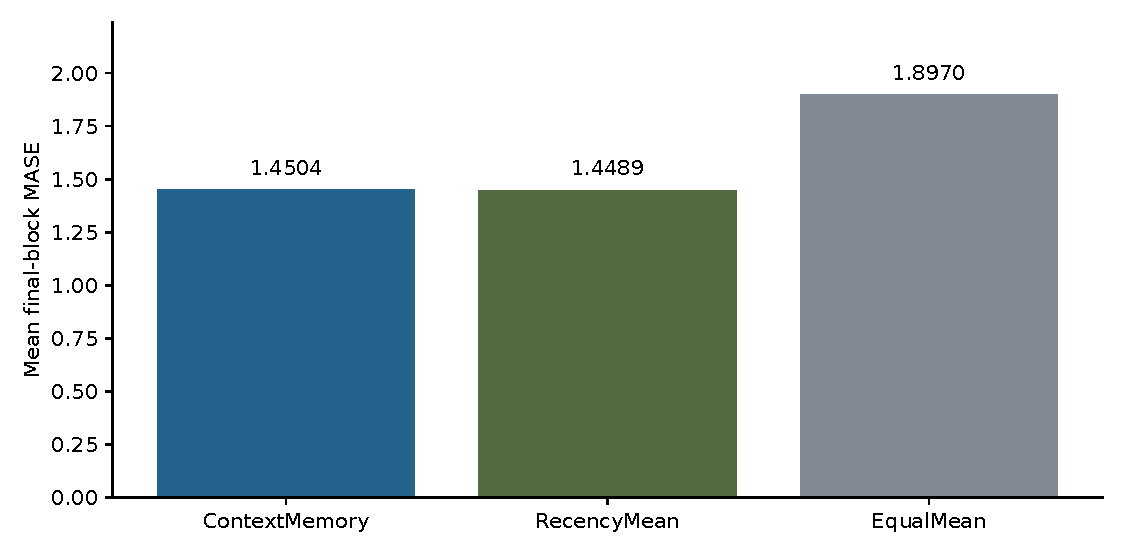
\includegraphics[width=0.87\textwidth]{proposal-comparison.pdf}
\caption{Fixed matching-expert combinations on the corrected fifteen-case protocol. Lower mean MASE is preferable. The contextual component does not improve on the recency-only ablation. Bars summarize selected final blocks, not independent population replications.}\end{figure}

\section{Measured final-block results}
\begin{longtable}{lrrr}
\caption{Corrected common final-block comparison on all fifteen selected cases. Each case has equal weight; coverage and scaled error describe this finite collection rather than a population guarantee.}\label{tab:archived-results}\\
\toprule Method & Cases & Mean MASE & Mean coverage\\\midrule\endfirsthead
\toprule Method & Cases & Mean MASE & Mean coverage\\\midrule\endhead
Chronos-Bolt & 15 & 1.0363 & 0.7563 \\
TimesFM-2.5 & 15 & 1.0633 & 0.8071 \\
TiRex-2 & 15 & 1.0809 & 0.7694 \\
Chronos-2 & 15 & 1.1555 & 0.6905 \\
DLinear & 15 & 1.1600 & 0.5595 \\
AutoARIMA & 15 & 1.2104 & 0.7813 \\
NLinear & 15 & 1.2298 & 0.4524 \\
NHITS (nf) & 15 & 1.2546 & 0.5079 \\
NHITS & 15 & 1.2898 & 0.4857 \\
LightGBM & 15 & 1.2983 & 0.5786 \\
SeasonalNaive & 15 & 1.4137 & 0.8702 \\
RecencyMean & 15 & 1.4489 & 0.8889 \\
ContextMemory & 15 & 1.4504 & 0.8944 \\
AutoTheta & 15 & 1.4964 & 0.7329 \\
HoltWinters & 15 & 1.6778 & 0.8639 \\
AutoETS & 15 & 1.6940 & 0.7639 \\
NLinear (nf) & 15 & 1.7547 & 0.1821 \\
EqualMean & 15 & 1.8970 & 0.8611 \\
SES & 15 & 1.9167 & 0.8274 \\
Theta & 15 & 1.9224 & 0.8274 \\
Holt & 15 & 3.9846 & 0.7302 \\
DLinear (nf) & 15 & 10.7385 & 0.4996 \\
\bottomrule
\end{longtable}


Chronos-Bolt has the smallest mean MASE in this selected, mixed-provenance comparison, followed by TimesFM 2.5 and TiRex-2. Their paths were not freshly refitted or regenerated for this experiment. No statistical significance, resource-normalized superiority or independence from pretraining data follows from that order. Method-specific training budgets and context limits remain part of the compared configurations.

Coverage exposes substantial differences that a point ranking conceals. Several neural paths have narrow intervals and low observed coverage. A broad interval can increase coverage at the expense of decision usefulness; coverage alone should not be optimized. Individual case outcomes and widths remain available in the artifact and workbench, including unfavorable neural and combination results.

\begin{figure}[htbp]\centering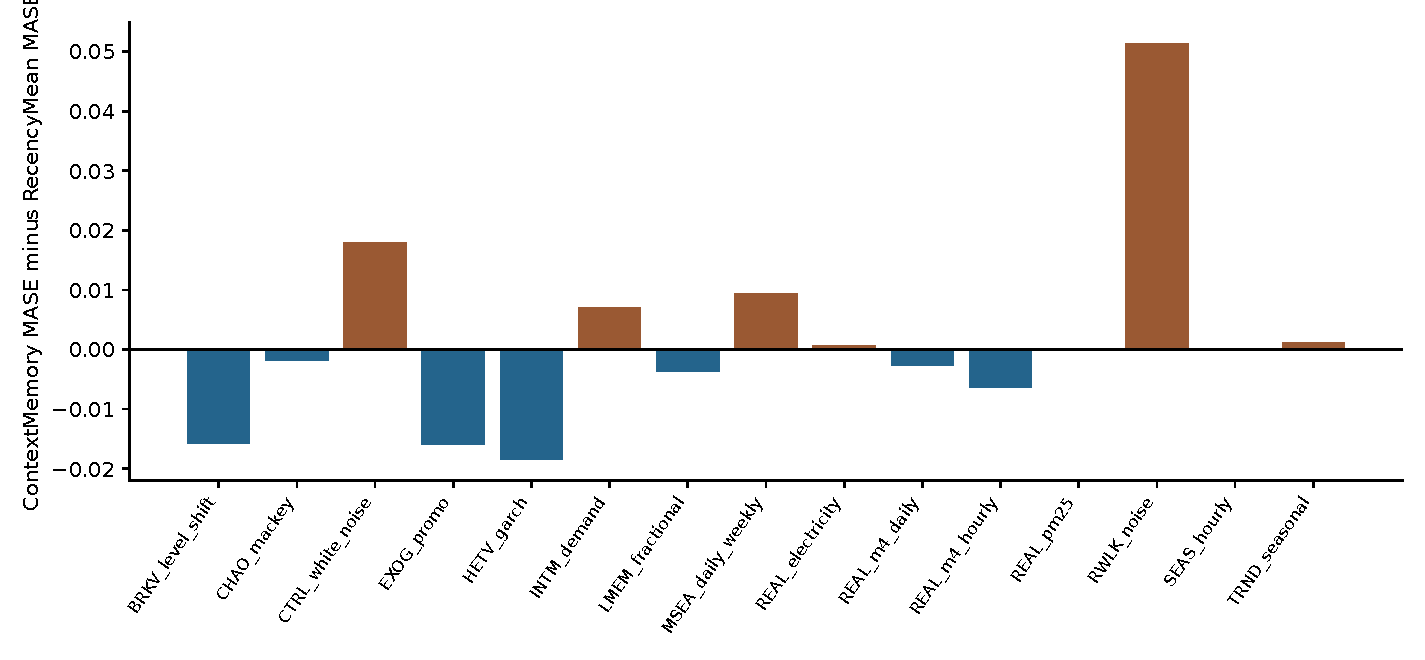
\includegraphics[width=\textwidth]{case-differences.pdf}
\caption{ContextMemory minus RecencyMean MASE for every selected case. Positive values favor the recency-only ablation. The common target and expert set isolate the contextual weighting component within each case, but the selected origins do not establish a general effect.}\end{figure}

ContextMemory's mean MASE is 1.4504, versus 1.4489 for RecencyMean. The difference is unfavorable at the declared primary criterion, despite occasional individual improvements. EqualMean gives 1.8970. Settings are unchanged after either the invalidated display-history calculation or the corrected run. A changed configuration would define a new experiment and must not overwrite this result.

\section{Streaming evaluation as separate evidence}
The committed streaming experiments use a predict--observe--update order inspired by prequential evaluation~\cite{dawid}. Their raw, adaptive conformal and PID-controlled intervals are evaluated along observation arrivals. Covariate availability is governed by an explicit known-future or lagged-past policy. These trajectories answer a different question from the final-block experiment and must not be pooled with its scores.

Adaptive conformal inference responds to distribution shift, while conformal PID control provides another adaptive mechanism~\cite{aci,pid}. Their assumptions and guarantees do not translate into conditional coverage for every local regime. Rolling coverage, width and adaptation delay should be read together. Original streaming timings are historical observations of their original runtime, rather than contemporary browser latency or a normalized hardware benchmark.

\section{Artifact and browser engineering}
Eight catalog boundaries cover traces, manifests, the index, diagnostic analysis, streaming results, ONNX metadata/assets, the corrected comparison and historical selector metadata. Normative JSON Schemas validate the committed JSON documents and generate browser TypeScript types through an OpenAPI component inventory. That inventory supports type generation without activating a prediction API. Cross-field invariants, source hashes, temporal reconstruction and numerical parity remain executable tests; a structural schema alone cannot enforce them.

The browser delegates chart interaction, summaries, tables, reset controls and keyboard support to the pinned shared shell. The product supplies data adapters, stable method identities and scenario state. Bilingual content uses locale-aware numbers; model and licence versions retain their identity. Request cancellation and generation identifiers prevent a slower case request or inference result from overwriting a newer selection.

Numbered local workflows check prerequisites, initialize declared environments, build an external data candidate and start the development server. Generation binds source and payload fingerprints, refuses partial inventories and changed frozen inputs, and separates candidate creation from explicit promotion. Historical engine-version metadata is retained rather than relabeled to match the new browser release. An unused epidemic-model surrogate inherited from an older repository structure was removed.

Eight executed English and Spanish notebooks progress through a seasonal reference, an incomplete-season experiment, actual statistical/tree adapter execution and the fixed combination with its ablations. Their metadata records exact direct dependencies, sources, inputs and method coverage. Fresh-kernel execution and byte comparison check that committed outputs are current. Numerical convergence notices are retained as portable text; machine paths and incidental notebook metadata are excluded.

\section{Validation and remaining scientific limits}
The validation layers are distinct. Structural schema checks establish artifact shape; source bindings establish input identity; independent equation tests establish selected numerical behaviours; browser traversal measures rendered routes and interactions; local notebook reproduction measures executable teaching artifacts. A successful build alone establishes none of the other layers. Computational records distinguish local numerical checks from remote CI, deployment and owner acceptance.

The main scientific limitations are: one origin per selected series; a small, non-random corpus; mixed fresh and frozen forecast provenance; unverified pretrained-data overlap; bounded historical training budgets; approximate lightweight uncertainty; possible numerical convergence issues in freshly executed reference adapters; and retrospective diagnostic artifacts that may include the final block. No operational acceptance or economic benefit is implied. A broader study should predeclare datasets, repeated origins, runtime and memory budgets, dependence-aware comparisons and independent pretraining-overlap checks.

For the contextual proposal, a stronger follow-up also needs faithful FFORMA and arbitrated-ensemble comparators rather than only internal ablations. Such work could reject or improve the proposed recurrence rule. The current negative outcome remains informative without being promoted to a general impossibility result.

\section{Reproduction and availability}
The source tree contains the corrected computation in \texttt{chronoscopelab.reevaluation}, the fixed proposal in \texttt{model/context\_memory.py}, original released traces, admitted source CSVs and the generated comparison. Running \texttt{scripts/reevaluate.py} regenerates the common final-block artifact while preserving the original traces. The staged local workflow provides complete candidate admission and explicit promotion. Exact commands, environment pins and validation results are recorded with the source.

The numerical tables and figures below are generated directly from the corrected artifact. Code and compact admitted data use the repository's software/data licences; prose uses the licence stated in the header. External publication, remote promotion and a verified live deployment are separate operations. Absence of those operations does not change a local numerical result, but prevents representing the candidate as a publicly delivered release.

\clearpage
\begin{thebibliography}{99}
\bibitem{theta} R. J. Hyndman and B. Billah, Unmasking the Theta method. \emph{International Journal of Forecasting}, 2003. \url{https://robjhyndman.com/papers/Theta.pdf}.
\bibitem{mase} R. J. Hyndman and A. B. Koehler, Another look at measures of forecast accuracy. \emph{International Journal of Forecasting}, 2006. \url{https://doi.org/10.1016/j.ijforecast.2006.03.001}.
\bibitem{scores} T. Gneiting and A. E. Raftery, Strictly proper scoring rules, prediction, and estimation. \emph{JASA}, 2007. \url{https://doi.org/10.1198/016214506000001437}.
\bibitem{fforma} P. Montero-Manso et al., FFORMA: Feature-based forecast model averaging. \emph{International Journal of Forecasting}, 2020. \url{https://doi.org/10.1016/j.ijforecast.2019.02.011}.
\bibitem{ade} V. Cerqueira et al., Arbitrated ensemble for time series forecasting. \emph{Machine Learning}, 2019. \url{https://doi.org/10.1007/s10994-018-05774-y}.
\bibitem{dawid} A. P. Dawid, Statistical theory: The prequential approach. \emph{JRSS A}, 1984. \url{https://doi.org/10.2307/2981683}.
\bibitem{aci} I. Gibbs and E. Cand\`es, Adaptive conformal inference under distribution shift. \emph{NeurIPS}, 2021. \url{https://arxiv.org/abs/2106.00170}.
\bibitem{pid} A. N. Angelopoulos, E. Cand\`es and R. J. Tibshirani, Conformal PID control for time series prediction. \url{https://arxiv.org/abs/2307.16895}.
\bibitem{fpp} R. J. Hyndman and G. Athanasopoulos, Forecasting: Principles and Practice. Holt--Winters seasonal method. \url{https://otexts.com/fpp3/holt-winters.html}.
\bibitem{statsforecast} Nixtla, StatsForecast model implementation documentation. \url{https://nixtlaverse.nixtla.io/statsforecast/src/core/models.html}.
\bibitem{chronos} Amazon Science, Chronos forecasting implementation and releases. \url{https://github.com/amazon-science/chronos-forecasting}.
\bibitem{timesfm} Google Research, TimesFM model API. \url{https://github.com/google-research/timesfm}.
\bibitem{tirex} TiRex-2 primary research record. \url{https://arxiv.org/abs/2607.01204}.
\end{thebibliography}
\end{document}
